\documentclass[dvipdfmx,autodetect-engine,titlepage]{jsarticle}
\usepackage[dvipdfm]{graphicx}
\usepackage{ascmac}
\usepackage{fancybox}
\usepackage{plistings}
\usepackage{itembkbx}
\usepackage{amsmath}
\usepackage{amssymb}
\usepackage{amsfonts}
\usepackage{svg}
\usepackage{url}
\usepackage{graphics}
\usepackage{multirow}
\usepackage{listings,jvlisting}

\textheight=23cm
\renewcommand{\figurename}{図}
\renewcommand{\tablename}{表}
\newenvironment{code}
{\vspace{0.5zw}\VerbatimEnvironment  
\begin{screen} 
\baselineskip=1.0\normalbaselineskip
 \begin{Verbatim}}
{\end{Verbatim}
\baselineskip=\normalbaselineskip
 \end{screen}\vspace{0.5zw}} 

\title{暗号理論(B1)\\最終レポート}
\author{山下 恭平\\学籍番号:2600200443-6}
\date{2023年1月19日}

\begin{document}

\maketitle

\section{AES(Advanced Encryption Standard)}


\subsection{AESとは}

AESとは「Advanced Encryption Standard」の略であり,アメリカが2000年に標準暗号と
して定めた共通鍵暗号アルゴリズムのことである.現在,実用化されている方式の中では,
強度が極めて高いといわれている.\begin{math}^{[1]}\end{math}

\subsection{作成の背景}

1977年に標準暗号として採用されたDES(Data Encryption Standard)にはいくつかの問題
が存在していたため,アメリカ国立標準技術研究所(NIST)の主導によって1997年に新しい標準暗号の
公募が行われた.そのため,「AES」は選出されなかった暗号も含む,手続き期間中から使われた
「新しい標準暗号」の総称であり,選出された暗号化方式の名前はRijndael(ラインダール)である.\begin{math}
  ^{[2]}
\end{math}
以下はNISTが公募した際の条件である

\begin{quote}
  \begin{itemize}
   \item 詳細なアルゴリズム仕様を公開すること
   \item ANSI C及びJavaによる実装を行うこと
   \item 128,192,256ビットの3通りの鍵長を利用できること
   \item ブロック長は128ビットであること
  \end{itemize}
 \end{quote}

 アルゴリズムの詳細を公開することは,RC4の暗号化アルゴリズムが当時は非公開だったものの,
 1994年に何者かによってアルゴリズムが漏洩させられたことが背景にあると考えた.RC4は
 現在でも利用されているが,特定の使用法によっては解読可能であることが示されているので,
 利用する際は注意をする必要がある.また鍵長が128bitから始まっているのは,以前標準であった
 DESは56bitの鍵長を採用しており,安全面においての不安要素が大きくなっていったからである.現在
 DESを単体で使用することは安全でないとされており,Triple DESという異なる3種類の鍵を用いて
 3回暗号化する方法が新たに開発されたが,既に理論的攻撃方法が存在しており,NISTによって
 2030年までには使用をやめるように警告が出されている.\begin{math}^{[3]}\end{math}

\subsection{Rijndael}

AESはJ.DaemenとV.Rijimen の提案したRijndaelという暗号化アルゴリズムを基に開発された.
AESの公募が行われた際に,NISTの示す条件を満たす暗号化方式が15個あったとされ,その中でも
優れた5方式が最終候補として残された,以下はその候補の一覧である.\begin{math}^{[2]}\end{math}

\begin{quote}
  \begin{itemize}
   \item Rijndael
   \item Serpent
   \item RC6
   \item Twofish
   \item Mars
  \end{itemize}
\end{quote}

 この中からRijndaelが採用された理由としては,高い暗号強度に加え,処理負荷や計算の速さでも
 高い評価を得ていたからである.

 \subsection{暗号アルゴリズム}

 AESが採用した暗号化アルゴリズムであるRijndaelについて簡単な解説を行う.まず図1
 にAESのアルゴリズムを示す.

\begin{figure}[h]
  \centering
  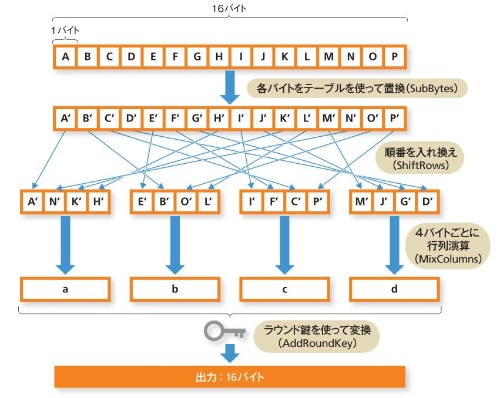
\includegraphics[scale=0.4]{fig1.jpg}
  \caption{暗号アルゴリズム(日経X TECH\begin{math}^{[4]}\end{math}より)}
\end{figure}

AESは4つのstepに分かれていることが確認できる.

\begin{enumerate}
  \item SubBytes(バイト交換)
  \item ShiftRows(行シフト置換)
  \item MixColumns(列変換)
  \item AddRoundKey(鍵加算)
\end{enumerate}

SubBytesでは16byteごとに区切ったデータに対し,1byte単位で置換が行われる.
次のShiftRowsではデータの各行に対して左巡回シフトを用いたデータ変換が行われる.
そしてMixColumnsではデータの各列に対してのデータ変換を行い,行列演算が行われる.
最後にAddRoundKeyでは,128ビット,192ビット,256ビットのいずれかの暗号鍵を基に
生成した鍵(ラウンド鍵)で変換を行う.以上がAESにおける暗号化の一連の流れである,
実際はこの演算が複数回繰り返して行われる.\begin{math}^{[4][5]}\end{math}

\subsection{安全性}
現在AESに対する最も有効的な攻撃の一つとしてBiclique攻撃が挙げられる.
この攻撃を使用することで,攻撃に必要となる計算回数が,AES-128に対しては
\begin{math}2^{126.1}\end{math}回,AES-192に対して\begin{math}2^{189.7}\end{math}回
,AES-256に対し\begin{math}2^{254.4}\end{math}回である.この数字から分かるように、
得られる計算削減量が僅かであることから,Biclique攻撃はAESにとって脅威となる攻撃では無い.
よってAESは2021年1月現在では極めて安全性能の高い暗号であることが分かる.また,今後
大きな計算削減を得られる攻撃手法が発見される可能性については専門家によっては懐疑的な
意見を示しており,今後長きにわたって利用可能だと考えられる.\begin{math}^{[6]}\end{math}


\section{TLS}

\subsection{TLSとは}

TLSとは(Transport Layer Security)の略称であり,インターネット上で行われる
コンピュータ同士がセキュリティが要求される通信を行うためのプロトコルである.
TLSはSSL(Secure Socket Layer)を基に標準化が行われており,SSL/TLSとも呼ばれる.
やりとりされるデータを暗号化し盗聴,漏洩,改竄を防ぐとともに,証明書によって通信を行っている相手が
正当なwebサイトの所収者であるかを判断し,なりすましを防ぐことができる.最も有名な使われ方の一つとして
HTTPS(HTTP over SSL/TLS)が挙げられ,webブラウザの上部に表示される鍵のマークはHTTPSで通信を
行っていることを示す.\begin{math}^{[7]}\end{math}

\subsection{作成の背景}

TLSの基となったSSLが初めてブラウザに実装されたのは1995年3月にリリースされたNetscape Navigator 1.1
である.この時実装されたのはSSL2.0であり,SSL1.0についてはプロトコルに重大な欠陥が発見されたため,
リリースされることはなかった.次にリリースされたSSL3.0がTLSの基となっており,1995年リリースされた.
現在ではTLS1.3までがリリースされており,SSL3.0については2014年に脆弱性が発見されたことから,
RFC7568によってSSL 3.0の使用は禁止されている.

\subsection{SSL/TLSの使用用途}

SSL/TLSは非常に多くの場面で利用されている,以下の表1はその一覧である.

\begin{table}[h]
  \centering
  \caption{over SSL/TLSが実装されてるプロトコル一覧}
  \begin{tabular}{|c|c|}
  \hline
  SSLと組み合わせたプロトコル & 元のプロトコル \\ \hline \hline
  HTTPS           & HTTP    \\ \hline
  SMTPS           & SMTP    \\ \hline
  LDAPS           & LDAP    \\ \hline
  FTPS            & FTP     \\ \hline
  IMAPS           & IMAP    \\ \hline
  POP3S           & POP3    \\ \hline
  \end{tabular}
\end{table}

この表から分かるように,webの閲覧をはじめファイル交換,メールの送受信など様々なサーバとの通信時
にTLSが利用されている.

\subsection{TLSハンドシェイクプロトコル}

クライアントとサーバの間がTCPによって接続された後にTLSハンドシェイクによって
通信の保護に取り掛かる.TLSハンドシェイクは大きく4つのフェーズに分けることができる.
以下にその4フェーズを簡潔にまとめる.\begin{math}^{[8][9]}\end{math}\\

\subsubsection*{第一フェーズ}
第一のフェーズではサーバ・クライアント間で通信に必要情報の合意を図る.このフェーズでは,
まずクライアントからサーバにClientHelloが送信され,次にサーバからクライアントにServerHello
が送信される.

\begin{enumerate}
  \item ClientHello
  \begin{itemize}
    \item[] クライアントがサーバーに「Hello」というメッセージを送信することによってハンドシェイクを開始する.
          これには,クライアントがサポートするTLSのバージョン,対応する暗号スイート,「クライアントランダム」
          というランダムなバイト文字列が含まれている.
  \end{itemize}
  \item ServerHello
  \begin{itemize}
    \item[] Client Helloメッセージへの返答として,サーバーがメッセージを送信する.
            これには,サーバーのSSL証明書,選んだ暗号スイート,サーバーが生成した別のバイト文字
            列「サーバーランダム」が含まれている.
  \end{itemize}
\end{enumerate}


\subsubsection*{第二フェーズ}

\begin{enumerate}
  \setcounter{enumi}{2}
  \item 認証
  \begin{itemize}
    \item[] クライアントはサーバーのSSL証明書を発行元の認証局へ確認を行う.
            これによってサーバーが自称する本人に間違いなく,クライアントはそのドメインの実際
            の所有者とやりとりしていることを確認することができる.
  \end{itemize}
\end{enumerate}

\subsubsection*{第三フェーズ}

\begin{enumerate}
  \setcounter{enumi}{3}
  \item プレマスタシークレット
  \begin{itemize}
    \item[] クライアントは「プレマスタシークレット」と呼ばれるランダムなバイト文字列
            をサーバへ送信する.この時,文字列はSSL証明書で得られた公開鍵で暗号化されており,
            復号はサーバが保有する秘密鍵でのみ行うことができる.
  \end{itemize}
  \item セッションキーの生成
  \begin{itemize}
    \item[] サーバは送られてきたプレマスタシークレットを解読する.その後,
            クライアントとサーバーは共にクライアントランダムとサーバーランダム,プレマスタ
            ーシークレットからセッションキーを生成する.双方とも同じ結果となれば成功.
  \end{itemize}
\end{enumerate}

\subsubsection*{第四フェーズ}

\begin{enumerate}
  \setcounter{enumi}{5}
  \item 準備完了
  \begin{itemize}
    \item[] サーバ,クライアントの双方が準備完了の合図として「finished」を送信する.
            これによってハンドシェイクが完了し,セッションキーを使用して通信が行われる.
  \end{itemize}
\end{enumerate}



% 参考文献はここに記述
\begin{thebibliography}{99}
    \bibitem{Otsuka}大塚商会. AES. 
      \url{https://mypage.otsuka-shokai.co.jp/contents/business-oyakudachi/words/aes.html} . (19/1/2023)
    \bibitem{Wiki}Wikipedia . Advanced Encryption Standard .『結城 暗号技術入門 第3版(2003: 69-71)』\\
      \url{https://ja.wikipedia.org/wiki/Advanced_Encryption_Standard#yuki2003} . (19/1/2023)
    \bibitem{Wiki}Wikipedia . Data Encryption Standard.\\
      \url{https://ja.wikipedia.org/wiki/Data_Encryption_Standard} . (19/1/2023)
    \bibitem{日経X}日経X TECH. 3分でわかるAES. 齊藤 貴之. \\
      \url{https://xtech.nikkei.com/atcl/nxt/keyword/18/00002/030800119/} . (19/1/2023)
    \bibitem{暗号の基礎}笠原正雄・佐竹賢治.『誤り訂正符号と暗号の基礎数理』. コロナ社. 2021
    \bibitem{解説論文}金子敏信 , 共通鍵暗号の安全性評価 , 電子情報通信学会 基礎・境界ソサイエティ Fundamentals Review 7巻 , 2013
    \bibitem{総務省}総務省. 国民のための情報セキュリティサイト.(19/1/2023) \\
      \url{https://www.soumu.go.jp/main_sosiki/joho_tsusin/security_previous/kiso/k01_ssl.htm} 
    \bibitem{Wiki}Wikipedia . Transport Layer Security. (19/1/2023)\\
      \url{https://ja.wikipedia.org/wiki/Transport_Layer_Security} 
    \bibitem{Cloudflare}Cloudflare . TLS/SSLハンドシェイクのプロセスは? (19/1/2023)\\
      \url{https://www.cloudflare.com/ja-jp/learning/ssl/what-happens-in-a-tls-handshake/#:~:text=TLS%E3%81%AF%E3%80%81%E3%82%A4%E3%83%B3%E3%82%BF%E3%83%BC%E3%83%8D%E3%83%83%E3%83%88%E9%80%9A%E4%BF%A1%E3%82%92,%E9%8D%B5%E3%81%AB%E3%81%A4%E3%81%84%E3%81%A6%E5%90%88%E6%84%8F%E3%81%97%E3%81%BE%E3%81%99%E3%80%82} 

\end{thebibliography}

\end{document}